%%----------------------------------------------------------------------
%%----------------------------------------------------------------------
\clearpage
\pagetitle{Organization}

\begin{columns}

This section describes how to conduct a \emph{Legacies} campaign, and
is mostly intended for the organizer.

\missionheading{Schedule}

Recon Squad games can be easily run in about~60 minutes in an event
setting with boards pre-arranged and armies unpacked before the clock
starts for each round.  Generally matches take at most~90 minutes even
at a very casual pace with no preparation beforehand.  The Cataclysm
game can be comfortably played in~4 hours including setup.  It's
therefore feasible to run \emph{Legacies} over either several
evenings, or a single full day.  A sample schedule for a single-day is:

\bigskip
\centerline{\begin{tabular}{cl}
11:00	 	& Doors open\\
11:50	 	& Registration Closes\\
12:00	 	& Campaign Briefing \& Alliance Pairings\\
12:15	 	& Round 1\\
1:25	 	& Alliance Pairings\\
1:35	 	& Round 2\\
2:40	 	& Alliance Pairings\\
2:50	 	& Round 3\\
3:50	 	& Alliance Pairings\\
4:00	 	& Round 4\\
5:00	 	& Dinner Break\\
5:30	 	& The Cataclysm\\
9:30	 	& Campaign Outcome \& Prizes\\
\end{tabular}}

\vfill

\noindent\fbox{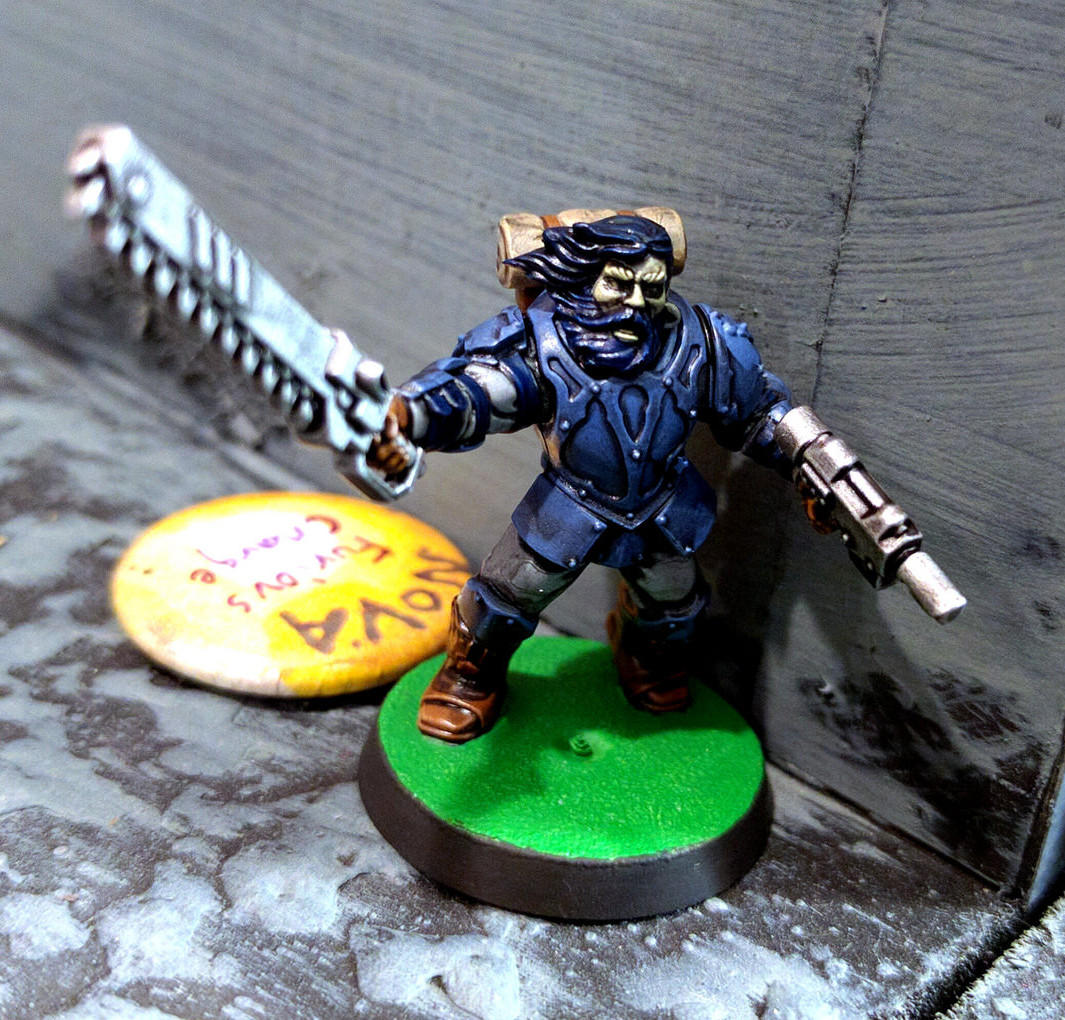
\includegraphics[width=\linewidth]{images/renegade-sgt-cropped.jpg}}

\columnbreak%

\missionheading{Alliances \& Story}

At the start of the campaign, the players are organized into two
alliances with an equal number of players.  In some groups this might
be faction specific, e.g., Chaos Daemons versus Eldar.  Generally
though an alliance will be comprised of several factions and can be
given a less specific title such as the Forces of Order, Legions of
Discord, or the Spoiler Horde.  How players are assigned alliances is
up to the organizer.  In a large event with mostly strangers and
tournament leanings it might be simply random.  In more
narrative-oriented and casual settings though, some attempt should be
made to take into account thematic cohesiveness as well as balanced
skill levels.

The concept behind the campaign is that each recon squad is a team of
veterans or other distinguished warriors tasked with several special
operations as part of a larger battle or war.  In the course of those
missions their paths eventually all cross, resulting in the larger
final battle.  Any specific background story is up to the organizer
and players, enabling a range of narratives with more or less detail.

\missionheading{Setup}

In advance of the campaign, players should be pointed to the Recon
Squad rules and the Missions section of this packet so they can design
their Recon Squad and Cataclysm army lists.  The campaign is themed
around players fielding a single Recon Squad list throughout, but the
organizer should feel free to be flexible about that requirement if
they wish.  In a campaign run over multiple days there is no need to
require Cataclysm lists be finalized until the last event.

Preparing for the campaign is very simple.  For each of the two
alliances, print and cut apart enough sets of the~8 legacy cards in
the Missions section to have at least one card per player.
Also print and cut apart enough sets of the~8 mission sheets to have
one for each match.  For a campaign with up to~16 players this means
making two sets of legacy cards and one set of mission sheets.

With anything but a very small number of players, it's probably easier
to have players record results separately from the mission sheets,
especially as the latter might be used again.  In that case, print and
cut apart enough copies of the scorecards at the end of this section
to have one for each match.  If using the scoring mechanism described
here, also print and cut apart enough copies of the ballots and
tickets to have one painting ballot per player and as many
sportsmanship tickets as might be necessary. Finally, print out one
copy of the Cataclysm scoresheet and as many copies of the players
scoresheet as needed.  A spreadsheet is available on the
\underline{\href{http://rocketshipgames.com/40k/legacies/}{\emph{Legacies}
    website}}.

\missionheading{Legacies}

After being assigned an alliance, each player chooses a legacy.  No
legacy may be selected twice within an alliance until all legacies
have been chosen at least once, and so on if there are even more
players.  Otherwise the alliance members may discuss among themselves
how to divy up the legacies.  If there is any contention, either ask
the players in random order to choose, or randomly assign legacies.

Each legacy lists three Recon Squad Missions and gives a Cataclysm
objective and legacy bonus.  To achieve their legacy, players must
accomplish the Cataclysm objective in the final team battle.  If they
win at least two of the three Recon Squad Missions in the given role
of attacker, defender, or either, then they receive their legacy bonus
in the Cataclysm.

Players' chosen legacies, match results, and whether or not they are
succeeding at their missions are all public information throughout the
campaign.

\missionheading{Round Pairings}

Recon Squad match pairings are made strategically by the alliances to
help their players achieve their legacy missions and further their
collective strategic goals.  Before each round, the alliances
alternate nominating one of their remaining unpaired players along
with a mission and role (attacker or defender).  The opposing alliance
then responds with a player for the match, who takes the other mission
role and chooses an unclaimed game board to play on.  This player must
be in the same or best similar win/draw/loss bracket as the nominated
player, unless the number of players is not great enough to make this
restriction without repeating match pairings.  In that case the later
rounds might require specific pairings to not have repeats.

For the first round, the initial alliance to put a player forward is
determined either randomly or based on the background story or the
outcomes of connected preceding events.  In subsequent rounds the
alliances alternate making the initial nomination.

\columnbreak
\noindent\fbox{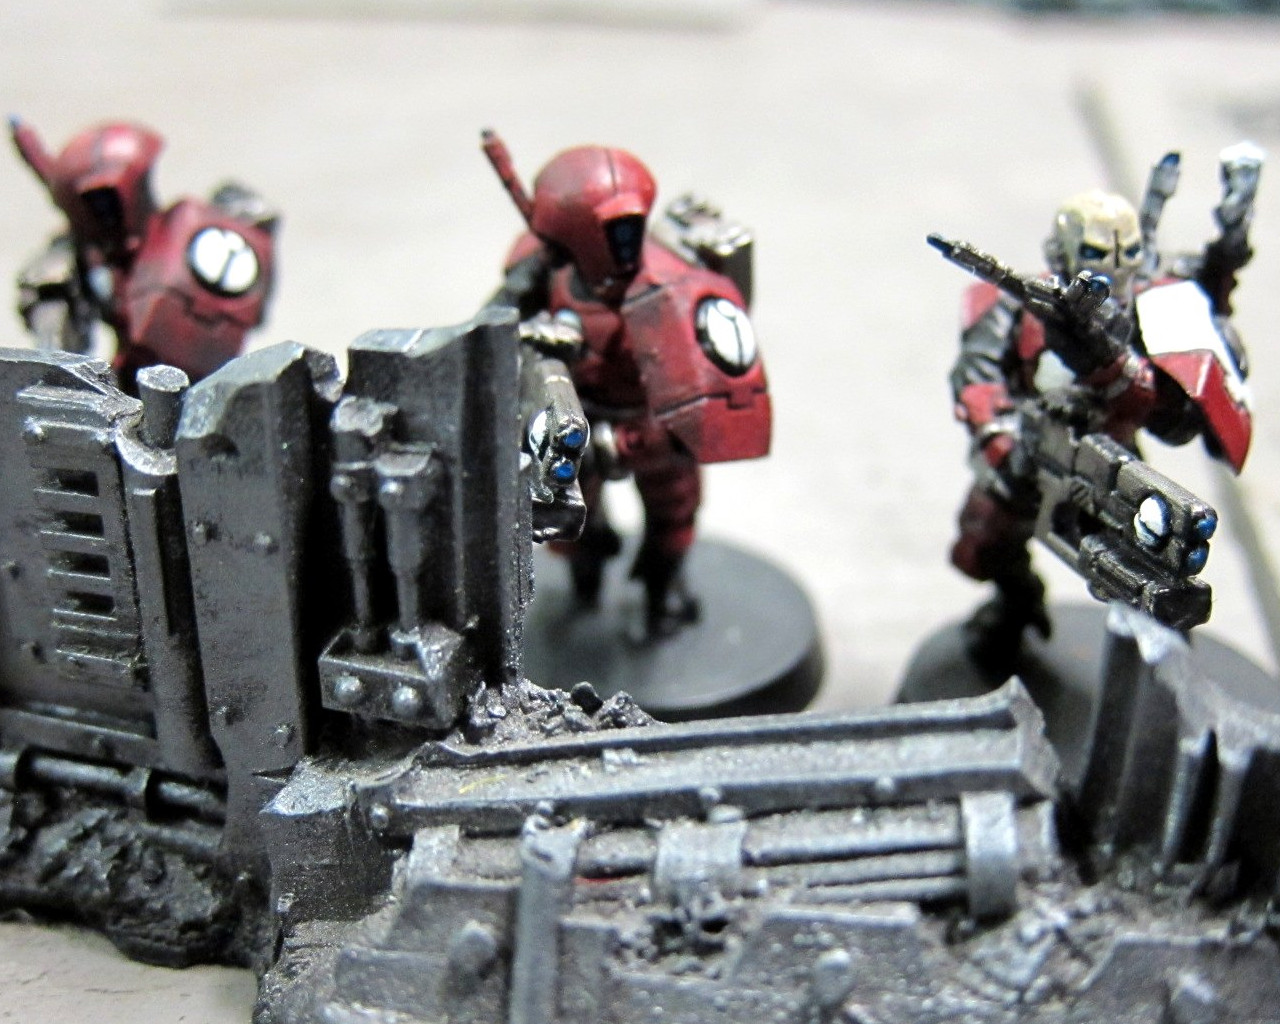
\includegraphics[width=\linewidth]{images/tau-line-cropped}}\\

%\vspace{12pt}
%\noindent\raisebox{0pt}[0.75in]{%
%\begin{minipage}{1.0\linewidth}  
\begin{story}{0.75in}{The Greater Good}
  Shas'ui Ke'ssai crouched behind the crude rubble barricade.  His
  hooves trembled with the clamorous approach of the humans' ugly,
  stinking, smoking vehicles.  In that moment, he realized he hated
  them.  He hated them for their violence, and he hated them for what
  they'd done to his world.  But most of all, he hated them for
  teaching him to hate.
\end{story}%
\bigskip

Players should use the checkboxes on their legacy cards to record
victories toward the Recon Squad Mission requirements, in addition to
the organizer keeping track.  It does not matter if the player was
nominated or the responding opponent, and they do not have to complete
the missions in any order.  In order to get their legacy bonus in the
Cataclysm they simply have to win each mission in the required role at
some point in the campaign.  Similarly, a player can attempt a mission
and role pair multiple times.  However, no advantage is gained by
winning the same mission and role pair multiple times.

\missionheading{Cataclysm}

Following the four rounds of Recon Squad games, the campaign concludes
by pitching the two teams against each other directly in the
Cataclysm.  Each player essentially adds 300 points to their Recon
Squad, as described in detail in the Missions section.


\missionsubheading{Board.}  The table for the Cataclysm game should be~4'
wide as usual, and roughly as many feet long as there are players in
the campaign.  So an~8-player campaign would conclude on an 8'x4'
table.  One idea to consider is simply moving together boards used in
the Recon Squad rounds, so that the battle thematically continues
directly over the same terrain.

\missionsubheading{Schedule.} The Cataclysm runs for a fixed 5 turns.
The organizer should determine and then enforce a schedule within the
time allotted for the match to ensure it completes, setting a specific
number of minutes for each turn.  Remember that later turns tend to go
faster as models have been removed.  A reasonable schedule of alliance
turns for a~4 hour period, accommodating setup, teardown, and scoring,
is:

\bigskip
\centerline{\begin{tabular}{cc}
Deployment & 15 minutes each\\
Turn 1& 20 minutes each\\
Turn 2& 20 minutes each\\
Turn 3& 15 minutes each\\
Turn 4& 15 minutes each\\
Turn 5& 10 minutes each\\
\end{tabular}}

\bigskip%
It is also important to ensure that enough time is reserved within
each alliance's turn to resolve the assault phase.  Players and armies
focused on close combat might otherwise be disadvantaged.  The
organizer should make sure alliances move on to the assault phase with
time to resolve combats as necessary, even if it means cutting short
their other actions.

\missionsubheading{Teams.}  All players in an alliance select and
field their own separate army lists following the rules given in the
Cataclysm mission.  For all gameplay purposes except as specifically
noted by the Cataclysm rules and mission, the combined forces of an
alliance are considered a single army comprised of multiple
detachments and the team a single player.

\missionsubheading{Allies.}  Regardless of factions, players consider
their teammates' models to be allies of convenience to their own army.
Interactions between a player's own models are governed by the allies
matrix as usual.

\missionsubheading{Turns.}  Alliance turns are player turns in all
ways.  Any actions not completed within turn time limits are
forfeited.  In game terms, each action happens sequentially as in a
standard game: One unit moves, then another, then the game proceeds to
the psychic phase and no more movements may be made, and so on.
However, in the interest of time, in practice players with no more
actions to take in a phase should carefully proceed to the subsequent
phase, provided there will be no effect on another player's remaining
actions in the current phase.  Alternatively, players without actions
of their own to complete should help execute actions of their
teammates, e.g., resolving multiple unrelated ongoing combats in
parallel.
%Time \emph{must} be reserved for the assault phase if there
%are ongoing combats.

\missionsubheading{Scope Limits.}  Special rules that affect all
units, all enemy units, or the entire table are not applied.  Specific
examples include the Chaos Daemons' Warp Storm table, the Lord of the
Storm rules for the Necron's Imotekh the Stormlord, and the Necron
Solar Pulse, none of which take effect.

Army-wide buffs apply only to that detachment of that player's forces,
as in a usual game, regardless of other factions that may be present
in the alliance.  For example, nominating Vulkan He'stan as a warlord
makes only that player's Melta weapons in Vulkan's detachment
Mastercrafted and does not affect any other detachments or players in
their alliance, including other Salamanders Space Marines.

\missionsubheading{Psychic Phase.}  In the psychic phase, a single D6
is rolled by the current alliance to determine the base warp charge
from which all of the players generate their own individual pools,
applying the usual rules to their own models.  Players all use their
own warp charge pool; teammates cannot combine or share warp charge.
Any opposing player with models on the table may attempt to deny the
witch, caveat that if a specific unit of enemy models is targeted,
their player alone may attempt to block the spell.

\missionsubheading{Objectives.} If units from multiple players in an
alliance control an objective marker, then each is considered to
control it for puposes of meeting the Cataclysm objective for their
legacy.  They do not all score though, alliance victory points are
only awarded once.

\vfill
\bigskip
\centerline{\fbox{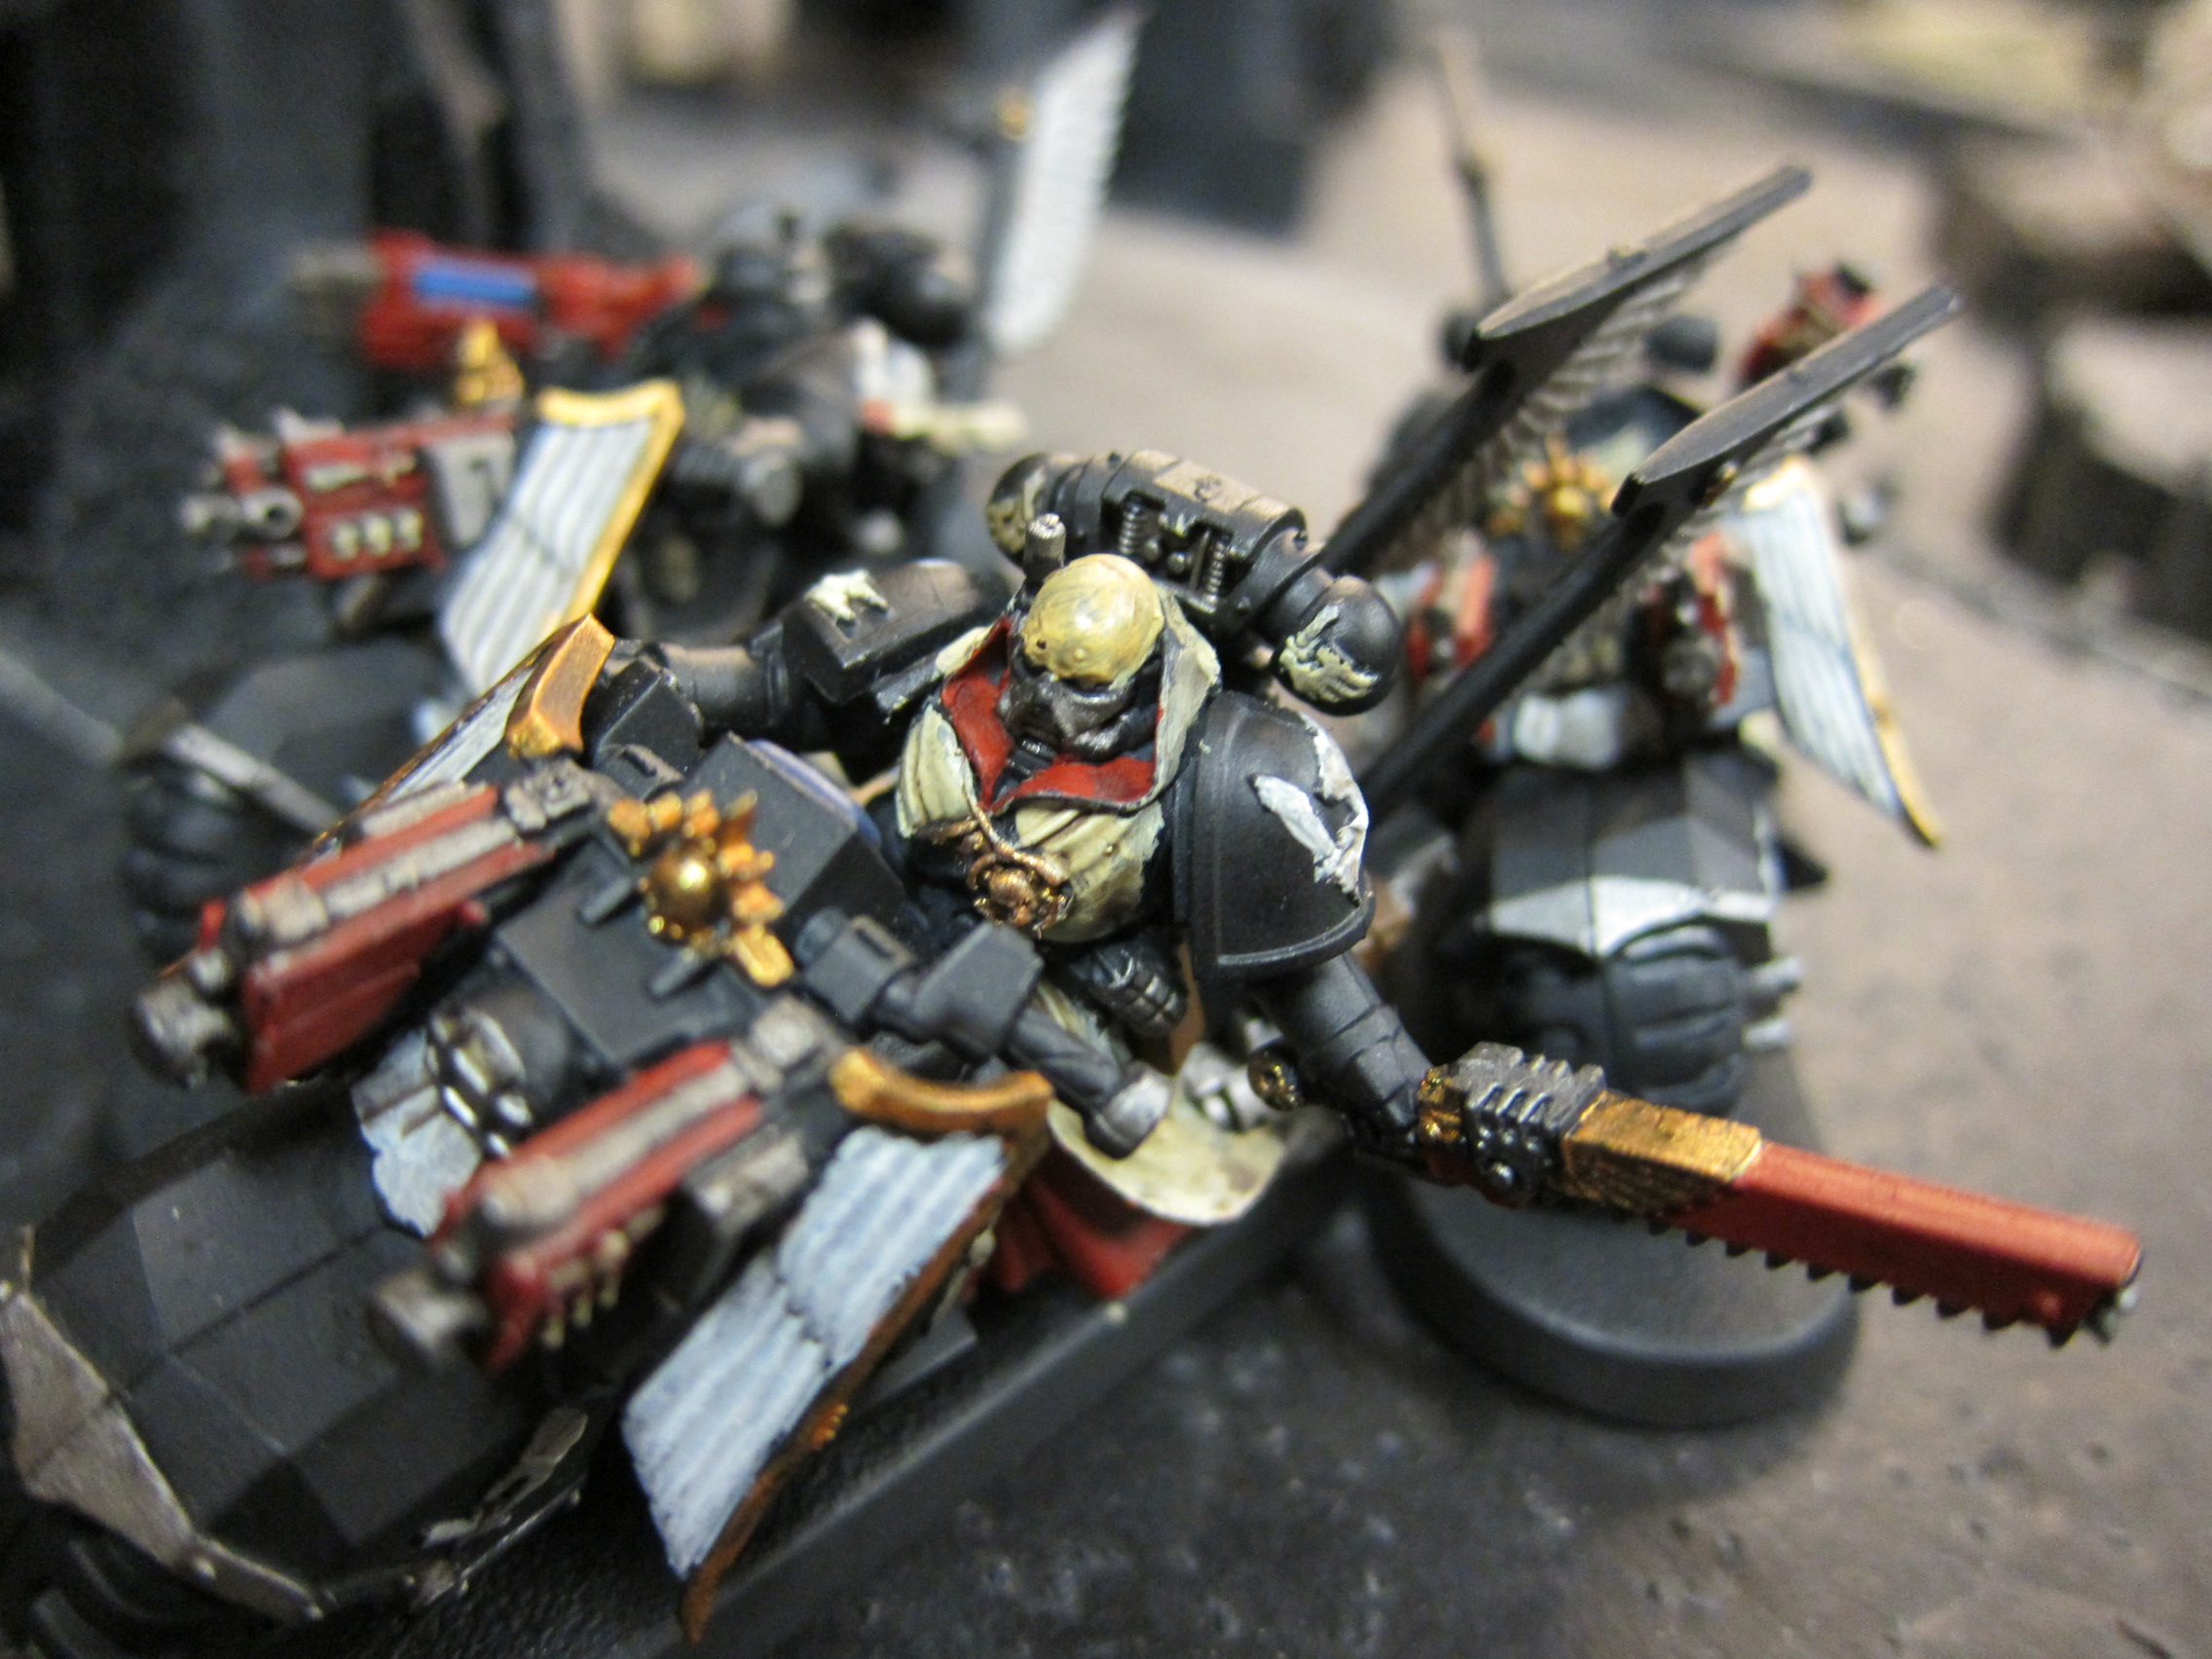
\includegraphics[width=\linewidth]{images/biker-sergeant}}}
\clearpage

\missionheading{Scoring and Prizes}

\emph{Legacies} is oriented to casual play but can easily be used for
a narrative tournament.  Prizes should be kept small and well
distributed though to limit the stakes, given that top players may not
face each other if they're in the same alliance, players don't all
contest the same scenarios, some missions are asymmetric, and so on.
There should also perhaps be two sets of prizes for any gameplay
awards, one for each alliance.  The following section outlines one
possible narrative tournament scoring and prize scheme.

\missionsubheading{Prizes.} Three prize categories are offered:

\begin{itemize}\shortlist
\item Winners in each alliance by overall scores;
\item Painting award based on player voting;
\item Best squad leader by top game results.
\end{itemize}

\missionsubheading{Overall Scores.} A total of~100 points are
available for each player throughout the campaign:

\begin{itemize}\shortlist
\item 60 points for game results;
\item 20 points for painting and craftsmanship;
\item 20 points for sportsmanship.
\end{itemize}

\missionsubheading{Game Results.} 

Each of the four Recon Squad missions are worth up to~12 points:

% Major victories award~10 points to the winner and 0 to the not-winner.
% Minor victories award~7 points to the winner and 3 to the not-winner.
% Draws award~5 points to both players.  Each mission has~2 bonus points
% available.

\begin{itemize}\shortlist
\item Major victory:~10 points winner, 0 not-winner;
\item Minor victory:~7 points winner, 3 not-winner;
\item Draw:~5 points to both players.
\item 2 bonus points are available in each mission.
\end{itemize}

%\begin{itemize}\shortlist
%\item Major victories award~10 points to the winner and 0 to the not-winner;
%\item Minor victories award~7 points to the winner and 3 to the not-winner;
%\item Draws award~5 points to both players.
%\item 2 bonus points are available in each mission.
%\end{itemize}

Players may also earn up to~12 points in the Cataclysm toward their
individual game results:
\begin{itemize}\shortlist
\item 7 points for winning their Cataclysm objective;
\item 3 points if they earned their legacy bonus;
\item 2 points if their alliance won a tactical victory in the
  Cataclysm (most victory points earned).
\end{itemize}

\columnbreak
\missionsubheading{Painting and Craftsmanship.} 

Painting and craft work is scored objectively by the organizer
applying this rubric to the entire army:

\begin{itemize}\shortlist
\item All models assembled and primed: \hfill +5 pts
\item All models three-color minimum: \hfill +5 pts
\item All models based (paint/flock): \hfill +4 pts
\item Advanced painting techniques present on any model (washes,
  drybrushing, etc.): \hfill +3 pts
\item Advanced basing techniques present on any model (3D details,
  varied flock, etc.): \hfill +3 pts
\end{itemize}

Note that this goes solely toward overall scores.  The painting award
is based purely on player voting.

%\columnbreak

%\end{minipage}
%}

%\vspace*{-4pt}

%\vspace*{-4pt}
\missionsubheading{Sportsmanship.}

By default players earn~5 points for sportsmanship in each Recon Squad
round.  However, they may be docked points for poor behavior by an
opponent submitting a sportsmanship ticket:

%\vspace*{-18pt}
\begin{itemize}\shortlist\setlength{\parskip}{0pt}\setlength{\itemsep}{2pt}
\item Openly hostile or rude: \hfill -3 pts
\item Unnecessarily competitive: \hfill -2 pts
\item Sloppy measuring, line of sight, or dice: \hfill -2 pts
\item Unreasonably late, slow, or inattentive: \hfill -1 pt
\item Significantly unfamiliar with rules:
  \hfill -1 pt
\item Not prepared with clear, typed army lists: \hfill -1 pt
\end{itemize}

%\vspace*{-18pt}
Hopefully few or no tickets need be submitted; it's perfectly
acceptable for players to not penalize opponents.  It should be
feasible to supply each player one ticket to start and only give out
more as needed.

\missionsubheading{Painting Award.}  The painting award is determined
by player voting, not the painting scores.  Each player must submit a
ballot of what they consider the top three best-made armies, excluding
themselves, awarding~3,~2, and~1 votes.  The most votes wins.

%\vfill\vbox to 0pt{}
\end{columns}

\vfill
%\centerline{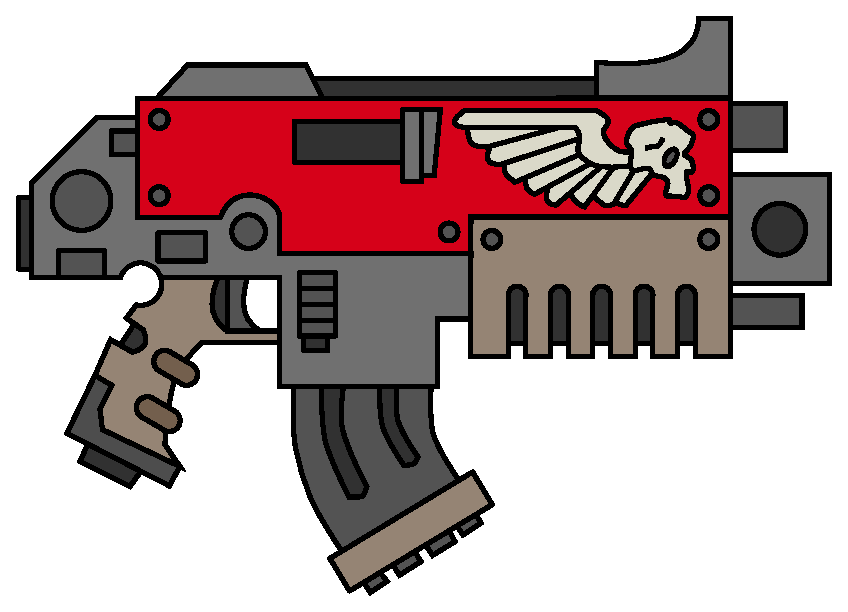
\includegraphics[width=0.6\linewidth]{art/bolter/boltgun}}

%\centerline{\fbox{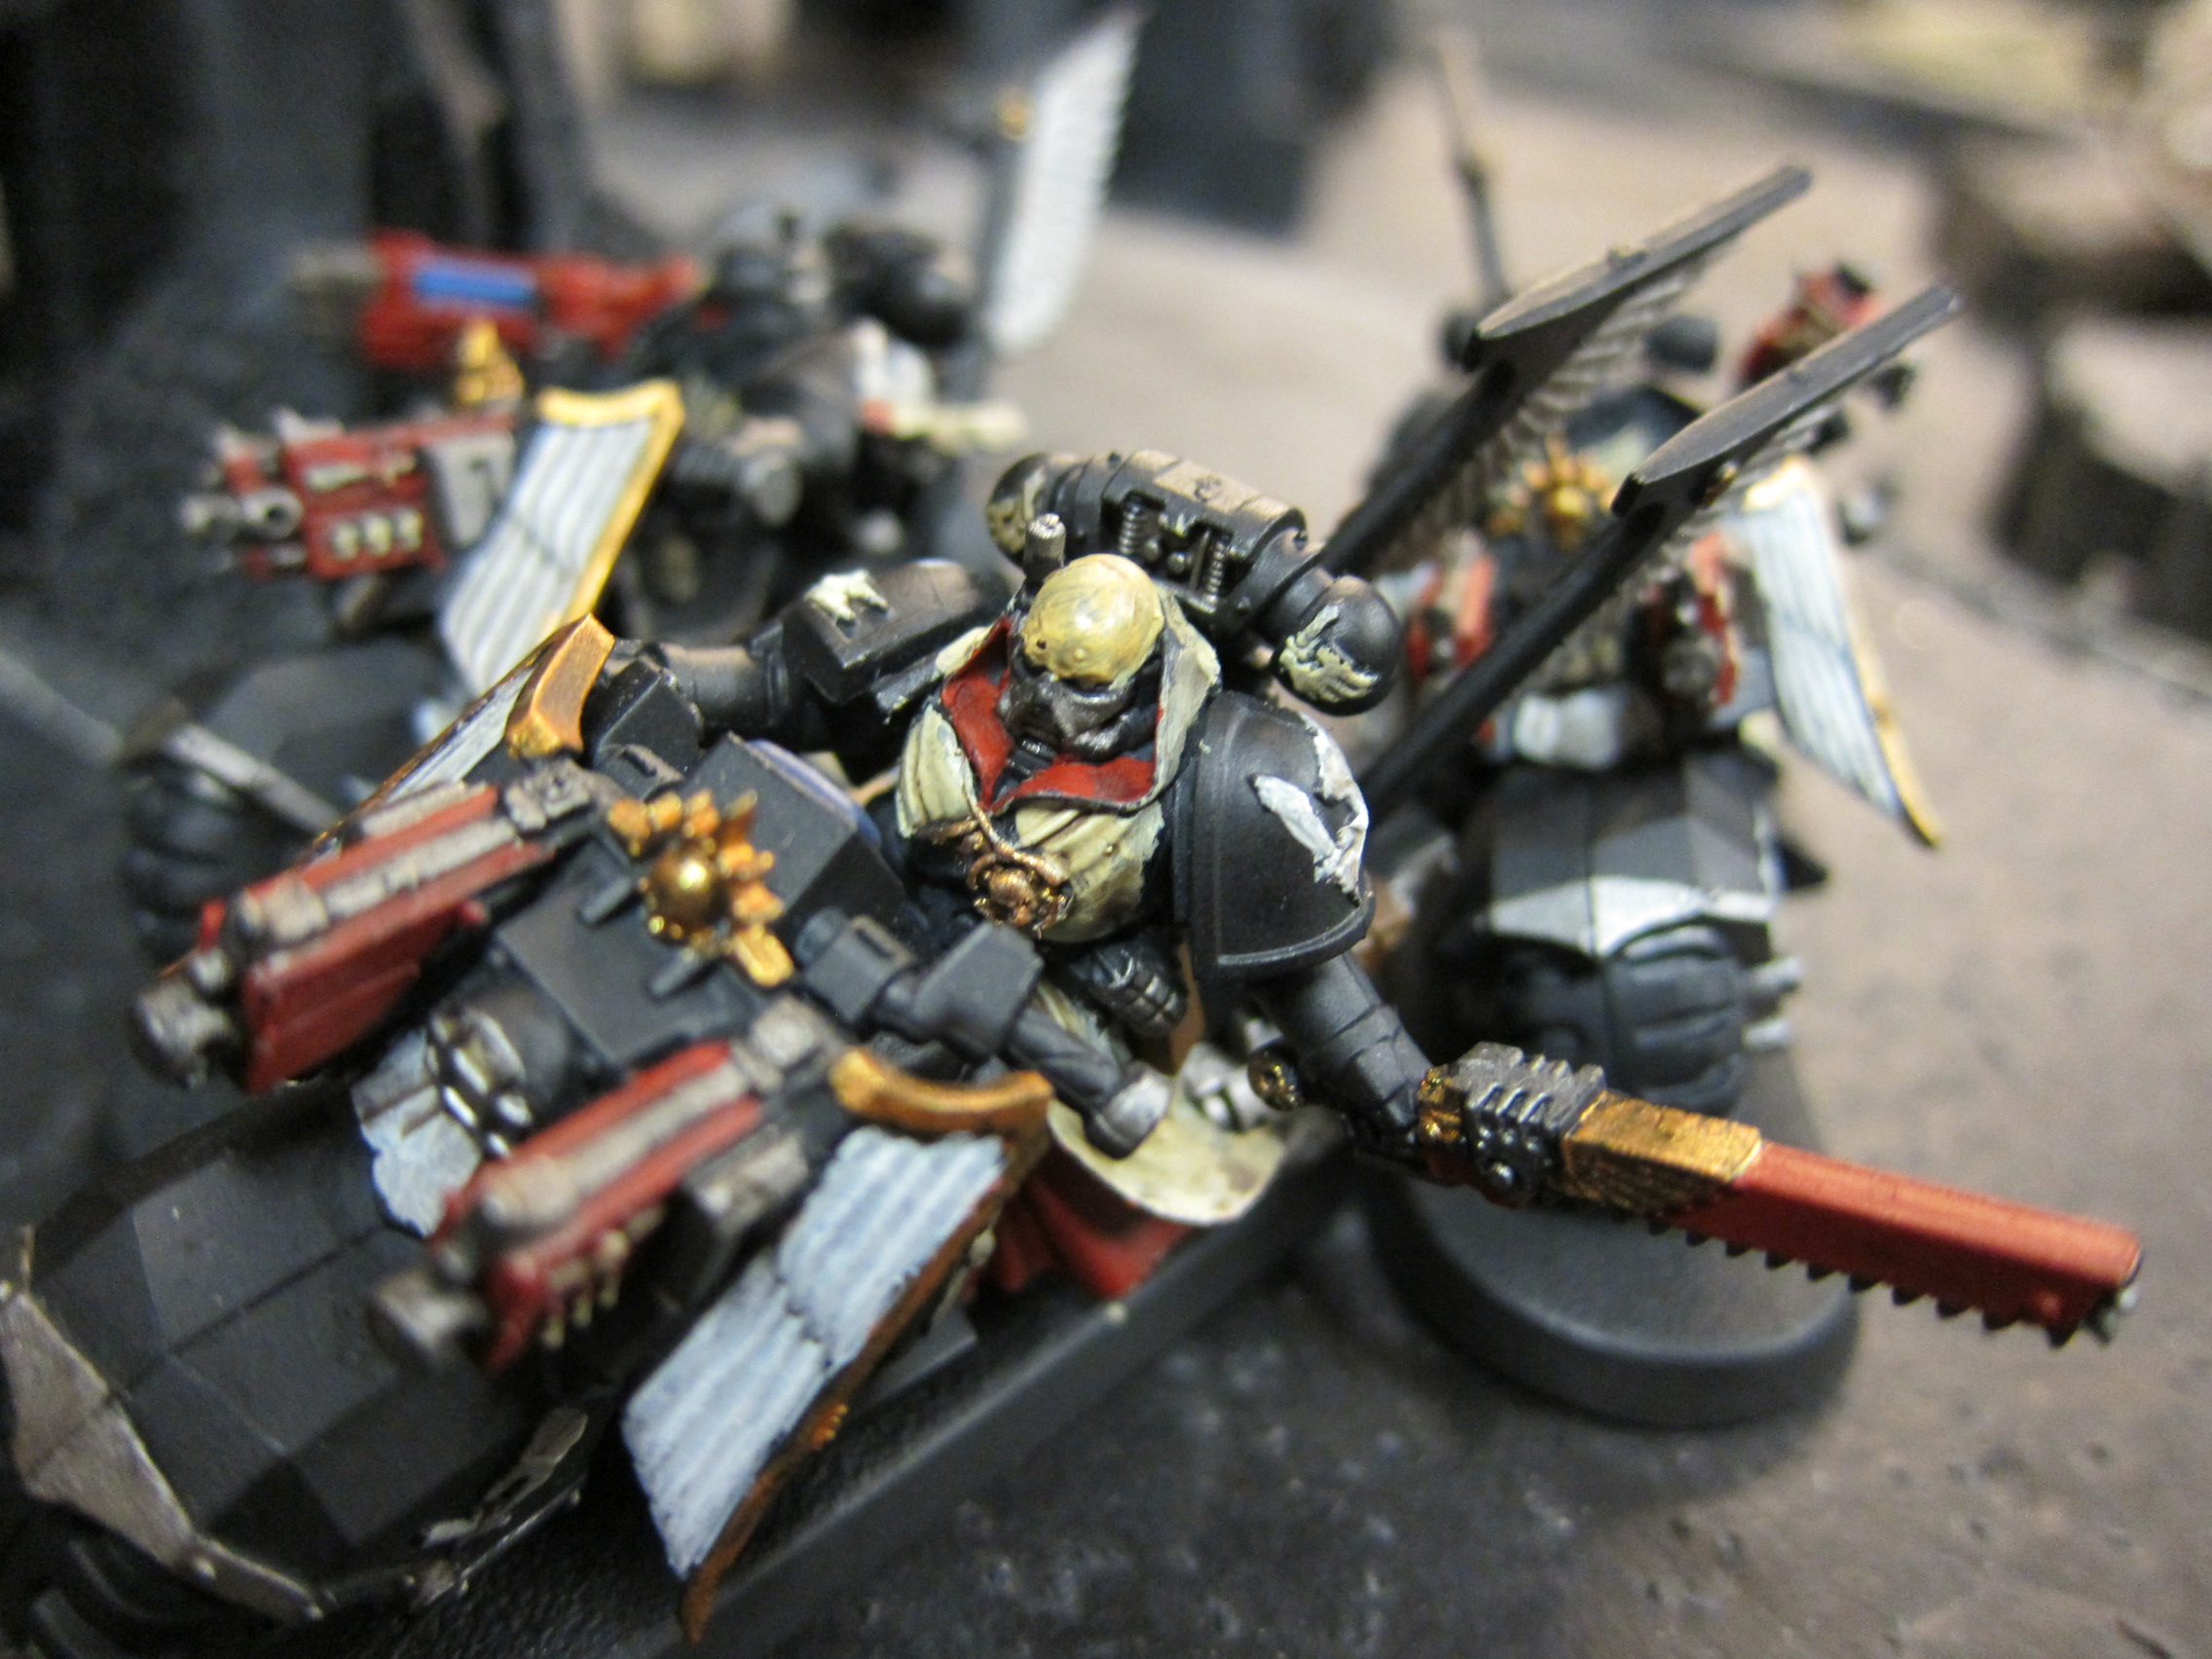
\includegraphics[width=0.5\linewidth]{images/biker-sergeant}}}
%\centerline{\fbox{\includegraphics[height=1.75in]{images/bloodangels-cropped}}}
\centerline{
\includegraphics[height=1.5in]{art/skulls}}
%\vfill\vbox to 0pt{}

\clearpage
\squelchbackground
\newcommand{\scorecard}{%
\begin{minipage}{3.25in}\centering
\begin{story}{62pt}{Game Results}
%\vspace*{2pt}

\vspace*{6pt}
{Attacker:}\raisebox{-4pt}{\hbox to 2.0625in{\enspace\hrulefill}}

\vspace*{8pt}
{Defender:}\raisebox{-4pt}{\hbox to 2in{\enspace\hrulefill}}

\vspace*{4pt}
\centering
\begin{minipage}{\linewidth}
{\vbox{\small%
\setlength{\tabcolsep}{2pt}%
\noindent\begin{tabularx}{\linewidth}{cccX}
  \raisebox{6pt}{\hbox to 1.25em{\rotatebox{15}{\small\bf Attacker}}}&
  \hbox to 1.25em{\rotatebox{15}{\small\bf Defender}}&
  &
  \multicolumn{1}{c}{\footnotesize\bf Outcome}
\\
  \hline
%
  \rescheck&\rescheck& & {\bf Major Victory}\\
%
  \rescheck&\rescheck& &
  {\bf Minor Victory}\\
%
\rescheck&\rescheck& &
{\bf Draw}\\
\hline \rescheck&\rescheck& &
{\bf Bonus Point}\\
\rescheck&\rescheck& &
{\bf Bonus Point}\\
\end{tabularx}%
}}%
\end{minipage}

\vspace*{9pt}
\vbox to 0pt{}

\end{story}
\end{minipage}
}

\clearpage
\begin{landscape}  
\noindent
\scorecard%
\hfill%
\scorecard%
\hfill%
\scorecard

\vfill

\noindent
\scorecard%
\hfill%
\scorecard%
\hfill%
\scorecard

\vfill

\noindent
\scorecard%
\hfill%
\scorecard%
\hfill%
\scorecard

\end{landscape}
\clearpage

%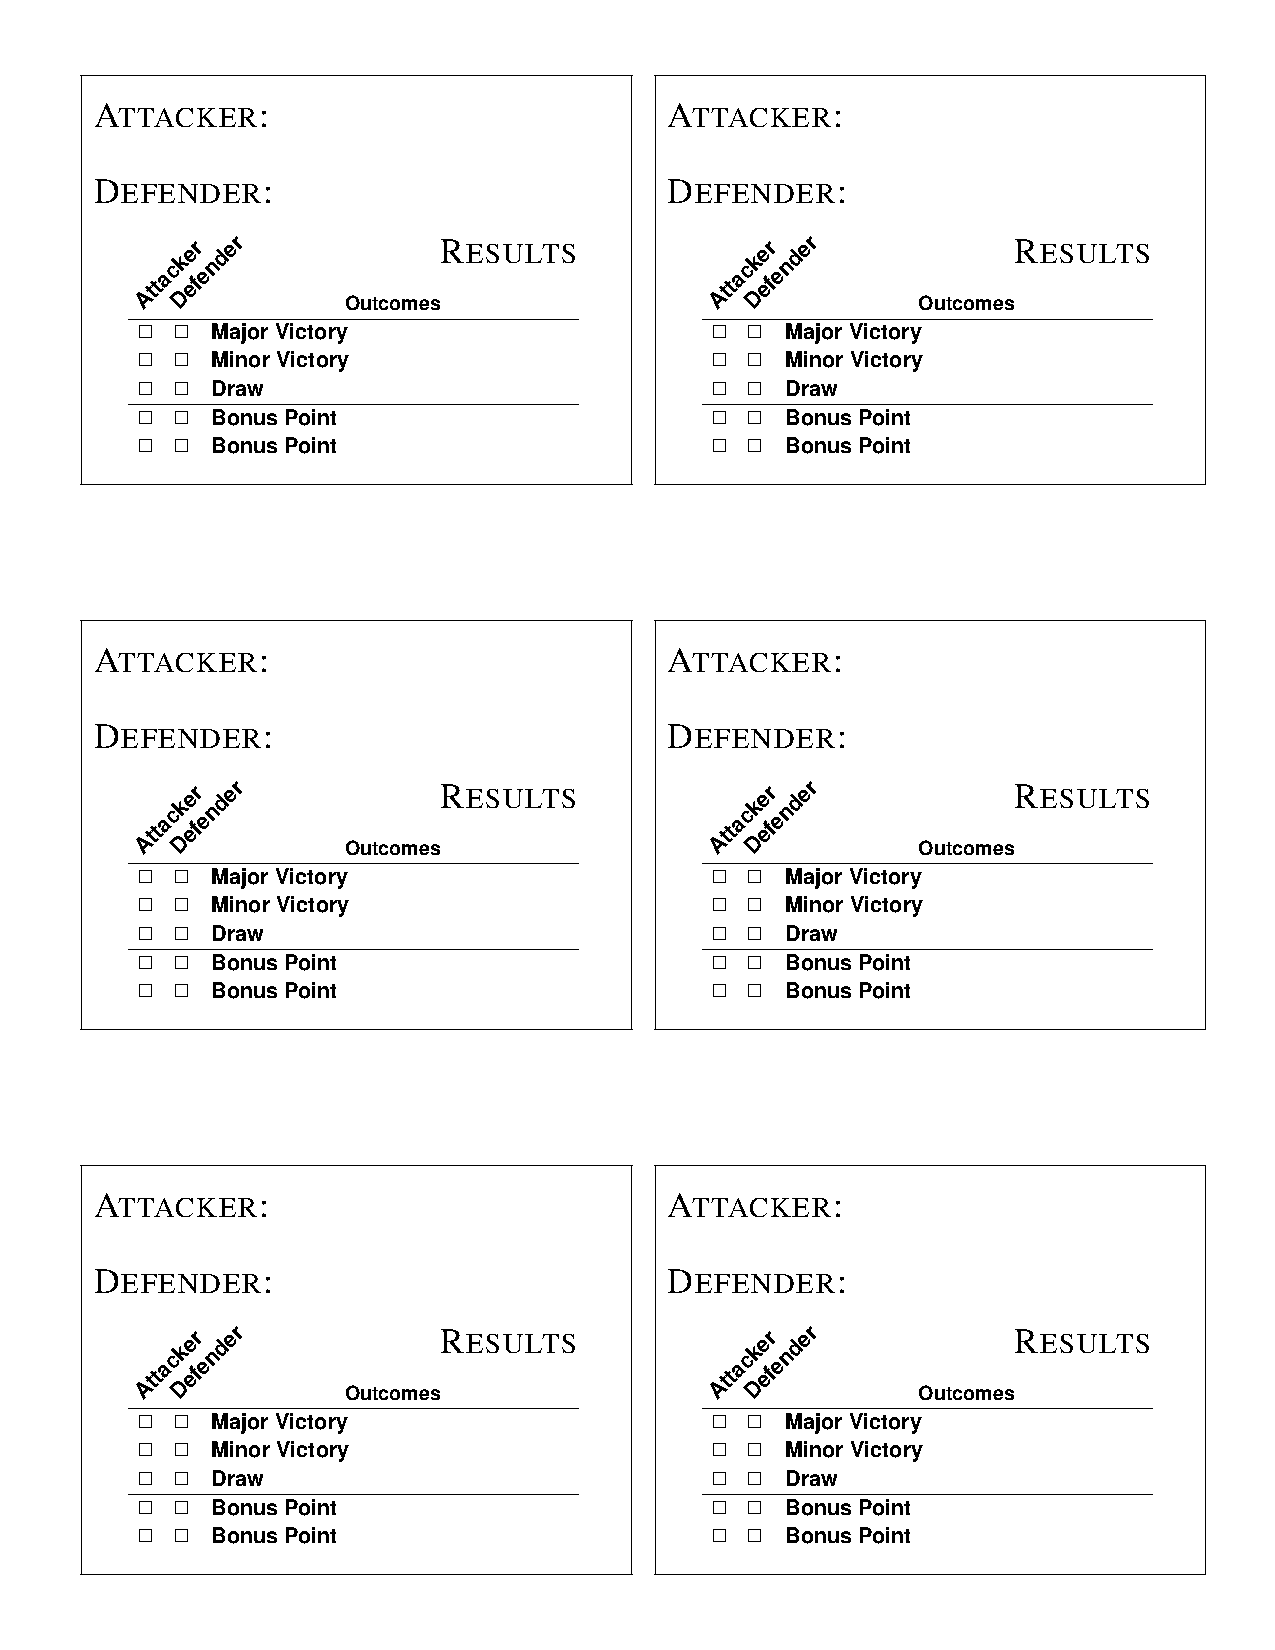
\includepdf[pages={1}]{20141220-scorecards.pdf}
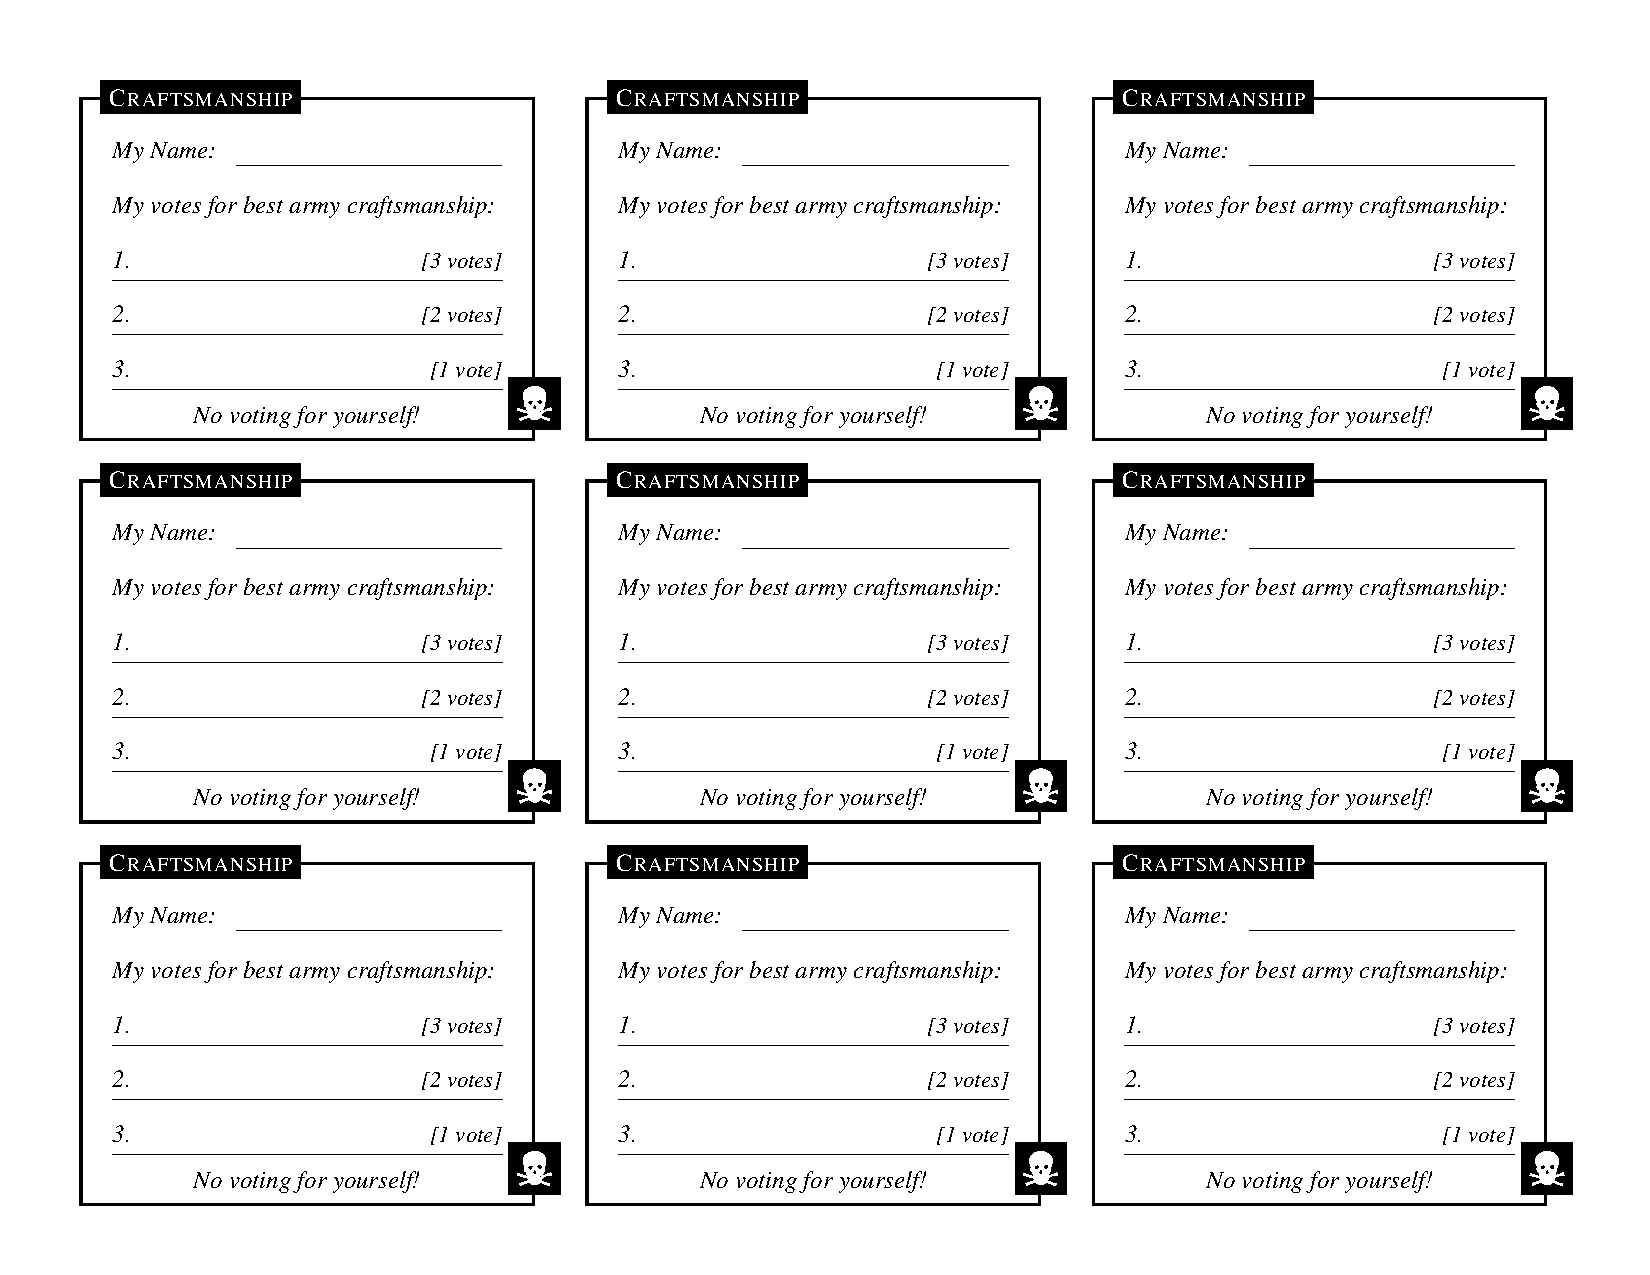
\includepdf[pages={1},landscape=true]{2016-painting.pdf}
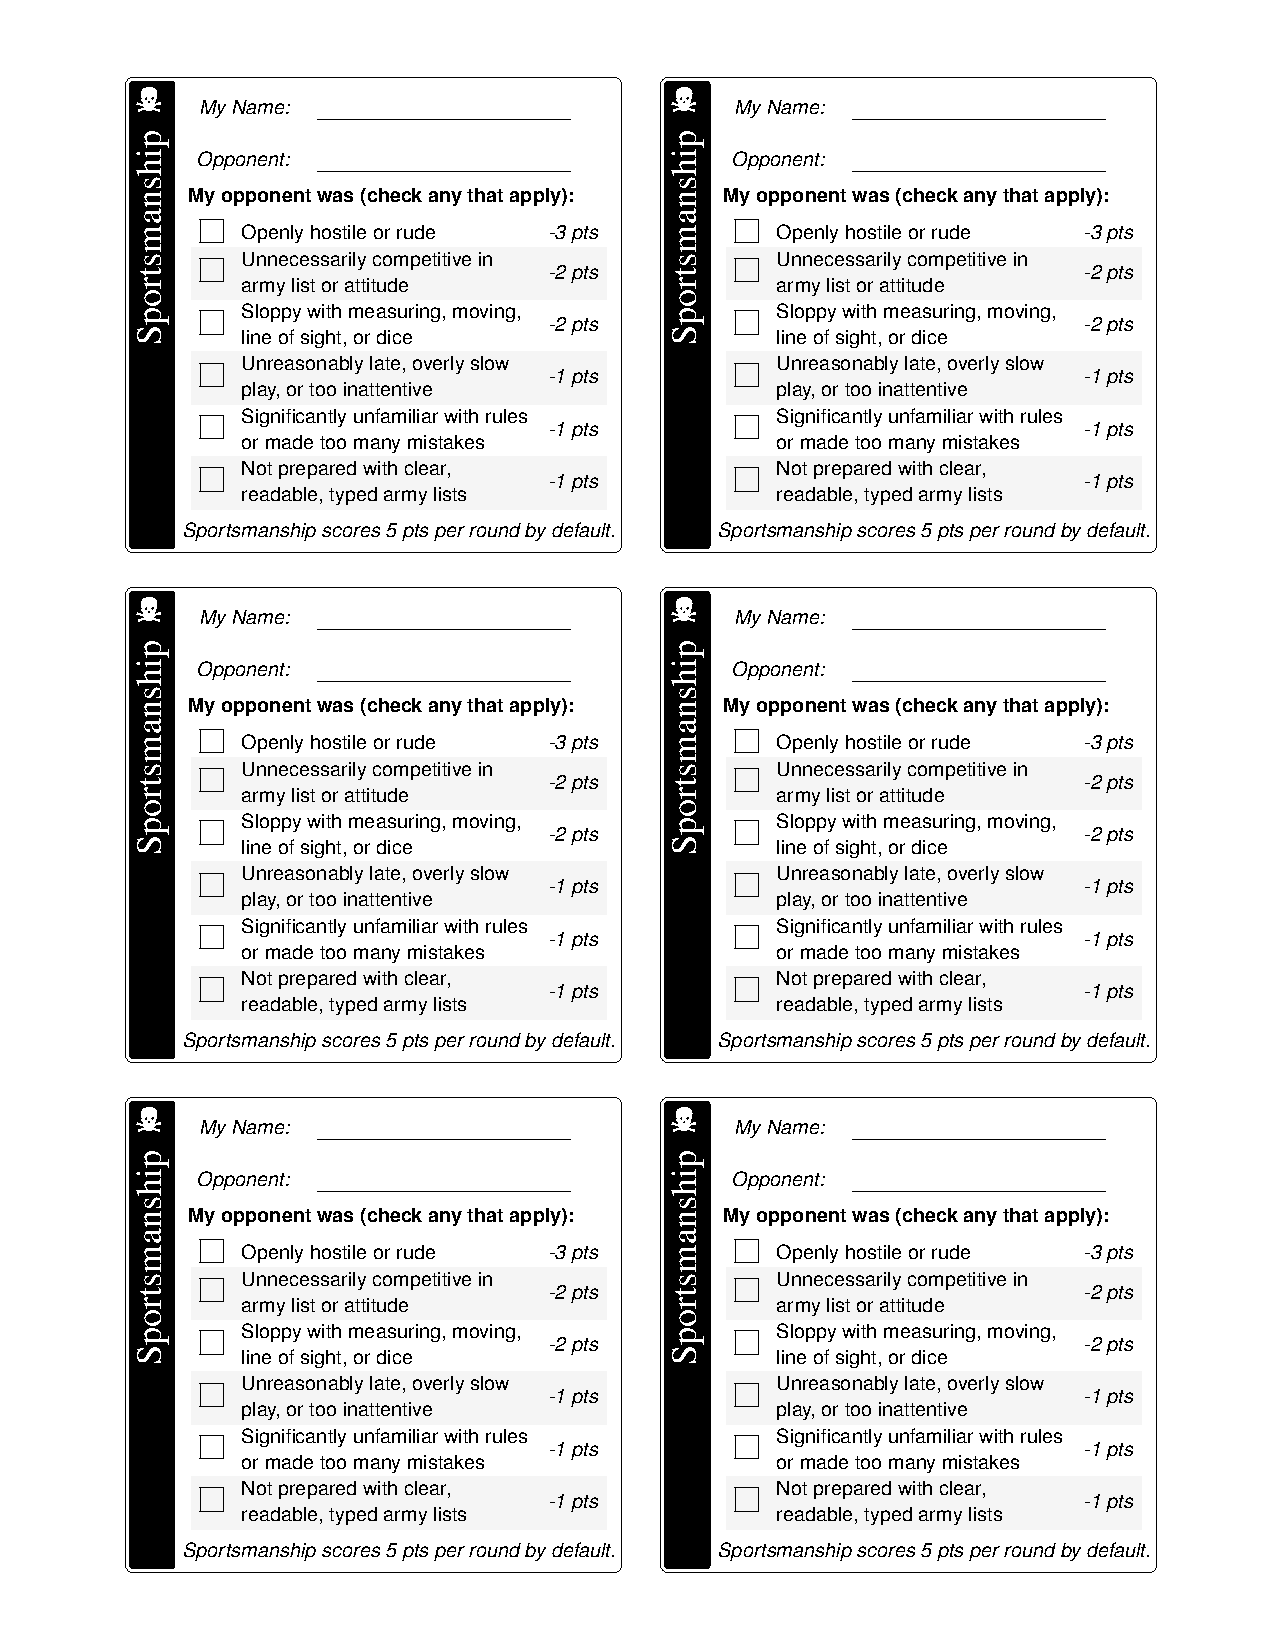
\includepdf[pages={1}]{2016-sportsmanship.pdf}

\clearpage
\thispagestyle{empty}
\section{Cataclysm Scoresheet}

\vfill
\centerline{
\rotatebox[origin=c]{90}{\textbf{Attacker Alliance: \raisebox{-4pt}{\hbox to 2.5in{\hrulefill}}}}~~~
\scalebox{0.9}{\fbox{
\begin{tabular}{rC{0.5in}cC{0.5in}cC{0.5in}cC{0.5in}cC{0.5in}cC{0.5in}}
& {\bf Turn 1}& & {\bf Turn 2}& & {\bf Turn 3}& & {\bf Turn 4}& & {\bf Turn 5}& & {\bf Total}\\
{\bf Primary} & \scorebox & + & \scorebox & + & \scorebox & + & \scorebox & + & \scorebox & = & \scorebox\\
& {\footnotesize\it (x1 pt)} & & {\footnotesize\it (x2 pts)} & & {\footnotesize\it (x3 pts)} & & {\footnotesize\it (x4 pts)} & & {\footnotesize\it (x5 pts)}&&\\
&&&&&&&&&&&\\
& {\bf Turn 1}& & {\bf Turn 2}& & {\bf Turn 3}& & {\bf Turn 4}& & {\bf Turn 5}& & {\bf Total}\\
{\bf Secondary} & \scorebox & + & \scorebox & + & \scorebox & + & \scorebox & + & \scorebox & = & \scorebox\\
& {\footnotesize\it (x1 pt)} & & {\footnotesize\it (x1 pt)} & & {\footnotesize\it (x1 pt)} & & {\footnotesize\it (x1 pt)} & & {\footnotesize\it (x1 pt)}&&\\
&&&&&&&&&&&\\
&& & \hbox to 32pt{\centerline{\bf Warmaster}}&  & \hbox to 32pt{\centerline{\bf Warlords}} & & {\bf First Blood} & & \hbox to 32pt{\centerline{\bf Linebreaker}}&&{\bf Total}\\
{\bf Tertiary} & & & \scorebox & + & \scorebox & + & \scorebox & + & \scorebox & = & \scorebox\\
& & & {\footnotesize\it (2 pts)} & & {\footnotesize\it (x1 pt)} & & {\footnotesize\it (1 pt)} & & {\footnotesize\it (1 pt)}&&\\
\hline
&&&&&&&&&&&\\[-12pt]
{\bf Total} &&&&&&&&&&&\scorebox\\
\end{tabular}
}}}

\vfill
\centerline{
\rotatebox[origin=c]{90}{\textbf{Defender Alliance: \raisebox{-4pt}{\hbox to 2.5in{\hrulefill}}}}~~~
\scalebox{0.9}{\fbox{
\begin{tabular}{rC{0.5in}cC{0.5in}cC{0.5in}cC{0.5in}cC{0.5in}cC{0.5in}}
& {\bf Turn 1}& & {\bf Turn 2}& & {\bf Turn 3}& & {\bf Turn 4}& & {\bf Turn 5}& & {\bf Total}\\
{\bf Primary} & \scorebox & + & \scorebox & + & \scorebox & + & \scorebox & + & \scorebox & = & \scorebox\\
& {\footnotesize\it (x1 pt)} & & {\footnotesize\it (x2 pts)} & & {\footnotesize\it (x3 pts)} & & {\footnotesize\it (x4 pts)} & & {\footnotesize\it (x5 pts)}&&\\
&&&&&&&&&&&\\
& {\bf Turn 1}& & {\bf Turn 2}& & {\bf Turn 3}& & {\bf Turn 4}& & {\bf Turn 5}& & {\bf Total}\\
{\bf Secondary} & \scorebox & + & \scorebox & + & \scorebox & + & \scorebox & + & \scorebox & = & \scorebox\\
& {\footnotesize\it (x1 pt)} & & {\footnotesize\it (x1 pt)} & & {\footnotesize\it (x1 pt)} & & {\footnotesize\it (x1 pt)} & & {\footnotesize\it (x1 pt)}&&\\
&&&&&&&&&&&\\
&& & \hbox to 32pt{\centerline{\bf Warmaster}}&  & \hbox to 32pt{\centerline{\bf Warlords}} & & {\bf First Blood} & & \hbox to 32pt{\centerline{\bf Linebreaker}}&&{\bf Total}\\
{\bf Tertiary} & & & \scorebox & + & \scorebox & + & \scorebox & + & \scorebox & = & \scorebox\\
& & & {\footnotesize\it (2 pts)} & & {\footnotesize\it (x1 pt)} & & {\footnotesize\it (1 pt)} & & {\footnotesize\it (1 pt)}&&\\
\hline
&&&&&&&&&&&\\[-12pt]
{\bf Total} &&&&&&&&&&&\scorebox\\
\end{tabular}
}}}


\clearpage
\thispagestyle{empty}
\section{Player Scoresheets}

\vfill
\noindent\begin{minipage}{0.5\linewidth}
\textbf{Player: \raisebox{-4pt}{\hbox to 2.5in{\hrulefill}}}  
\end{minipage}%
\begin{minipage}{0.5\linewidth}\raggedleft
\textbf{Alliance: \raisebox{-4pt}{\hbox to 2.5in{\hrulefill}}}
\end{minipage}

\smallskip
\centerline{\fbox{
\begin{tabular}{rC{0.5in}cC{0.5in}cC{0.5in}cC{0.5in}cC{0.5in}cC{0.5in}}
& \hbox to 32pt{\centerline{\bf Rnd 1}} & & \hbox to 32pt{\centerline{\bf Rnd 2}} & & \hbox to 32pt{\centerline{\bf Rnd 3}} & & \hbox to 32pt{\centerline{\bf Rnd 4}} & & \hbox to 32pt{\centerline{\bf Cataclysm}} & & {\bf Total}\\
{\bf Missions} & \scorebox & + & \scorebox & + & \scorebox & + & \scorebox & + & \scorebox & = & \scorebox\\
& \multicolumn{7}{c}{\parbox{3.25in}{\centering\footnotesize\it (major victory 10pts/loss 0pts; minor victory 7pts/loss 3pts; draw 5pts/5pts; 2 bonus points available)}}  & \multicolumn{3}{c}{\parbox{1in}{\centering\footnotesize\it (7pts obj. + 3pts leg. + 2pts win)}} & \\
&&&&&&&&&&&\\[-12pt]
& \hbox to 32pt{\centerline{\bf Rnd 1}} & & \hbox to 32pt{\centerline{\bf Rnd 2}} & & \hbox to 32pt{\centerline{\bf Rnd 3}} & & \hbox to 32pt{\centerline{\bf Rnd 4}} & & & & {\bf Total}\\
{\bf Sportsmanship} & \scorebox & + & \scorebox & + & \scorebox & + & \scorebox & &  & = & \scorebox\\
& {\footnotesize\it (5 pts)} & & {\footnotesize\it (5 pts)} & & {\footnotesize\it (5 pts)} & & {\footnotesize\it (5 pts)} & & &&\\
&&&&&&&&&&&\\[-12pt]
& \hbox to 32pt{\centerline{\bf Assembled}} &  & \hbox to 32pt{\centerline{\bf 3-Color}} & & \hbox to 32pt{\bf Based} & & \hbox to 32pt{\centerline{\bf Adv. Paint}} & & \hbox to 32pt{\centerline{\bf Adv. Base}} &&{\bf Total}\\
{\bf Painting} & \scorebox & + & \scorebox & + & \scorebox & + & \scorebox & + & \scorebox & = & \scorebox\\
& {\footnotesize\it (5 pts)} & & {\footnotesize\it (5 pts)} & & {\footnotesize\it (4 pts)} & & {\footnotesize\it (3 pts)} & & {\footnotesize\it (3 pts)} &&\\
\hline
&&&&&&&&&&&\\[-12pt]
{\bf Total} &&&&&&&&&&&\scorebox\\
\end{tabular}
}}

\vfill
\noindent\begin{minipage}{0.5\linewidth}
\textbf{Player: \raisebox{-4pt}{\hbox to 2.5in{\hrulefill}}}  
\end{minipage}%
\begin{minipage}{0.5\linewidth}\raggedleft
\textbf{Alliance: \raisebox{-4pt}{\hbox to 2.5in{\hrulefill}}}
\end{minipage}

\smallskip
\centerline{\fbox{
\begin{tabular}{rC{0.5in}cC{0.5in}cC{0.5in}cC{0.5in}cC{0.5in}cC{0.5in}}
& \hbox to 32pt{\centerline{\bf Rnd 1}} & & \hbox to 32pt{\centerline{\bf Rnd 2}} & & \hbox to 32pt{\centerline{\bf Rnd 3}} & & \hbox to 32pt{\centerline{\bf Rnd 4}} & & \hbox to 32pt{\centerline{\bf Cataclysm}} & & {\bf Total}\\
{\bf Missions} & \scorebox & + & \scorebox & + & \scorebox & + & \scorebox & + & \scorebox & = & \scorebox\\
& \multicolumn{7}{c}{\parbox{3.25in}{\centering\footnotesize\it (major victory 10pts/loss 0pts; minor victory 7pts/loss 3pts; draw 5pts/5pts; 2 bonus points available)}}  & \multicolumn{3}{c}{\parbox{1in}{\centering\footnotesize\it (7pts obj. + 3pts leg. + 2pts win)}} & \\
&&&&&&&&&&&\\[-12pt]
& \hbox to 32pt{\centerline{\bf Rnd 1}} & & \hbox to 32pt{\centerline{\bf Rnd 2}} & & \hbox to 32pt{\centerline{\bf Rnd 3}} & & \hbox to 32pt{\centerline{\bf Rnd 4}} & & & & {\bf Total}\\
{\bf Sportsmanship} & \scorebox & + & \scorebox & + & \scorebox & + & \scorebox & &  & = & \scorebox\\
& {\footnotesize\it (5 pts)} & & {\footnotesize\it (5 pts)} & & {\footnotesize\it (5 pts)} & & {\footnotesize\it (5 pts)} & & &&\\
&&&&&&&&&&&\\[-12pt]
& \hbox to 32pt{\centerline{\bf Assembled}} &  & \hbox to 32pt{\centerline{\bf 3-Color}} & & \hbox to 32pt{\bf Based} & & \hbox to 32pt{\centerline{\bf Adv. Paint}} & & \hbox to 32pt{\centerline{\bf Adv. Base}} &&{\bf Total}\\
{\bf Painting} & \scorebox & + & \scorebox & + & \scorebox & + & \scorebox & + & \scorebox & = & \scorebox\\
& {\footnotesize\it (5 pts)} & & {\footnotesize\it (5 pts)} & & {\footnotesize\it (4 pts)} & & {\footnotesize\it (3 pts)} & & {\footnotesize\it (3 pts)} &&\\
\hline
&&&&&&&&&&&\\[-12pt]
{\bf Total} &&&&&&&&&&&\scorebox\\
\end{tabular}
}}


\clearpage
\restorebackground
